\documentclass{article}
\usepackage[utf8]{inputenc}

\title{Report.6.map.tex}
\author{gw.muraro}
\date{November 1st 2018}

\usepackage{natbib}
\usepackage{graphicx}
\usepackage{pgfplots}
\usepackage{minted}

\begin{document}

\maketitle
\section{Labwork 6}

\subsection{Explain how you implement the labworks}
    
    The three CPU functions (labwork6\_GPU\_binarization, labwork6\_GPU\_brightness and labwork6\_GPU\_blending) are pretty much the sames, they just call different kernel functions. for these labworks, we are only going to explain the kernel function, since, the CPU function are explained into the previous labworks. 
    
    \begin{enumerate}     

    \item \textbf{Binarization}
    \newline Binarization is a process to make a pixel white or black with a threshold which is 128. In order to implement it, wi can use a simple condition : 
    \begin{minted}{c}
    if (input[tid].x < 128)
        [...]
    else 
        [...]
    \end{minted}
    
    But this condition will slow down the threads because of the "else". So we have to avoid it by using the integer division that can return 0 if the result is not greater than 1.0. So this is how the kernel is implemented :
    
    \begin{minted}{c}
__global__ void binarization(
    uchar3 *input, 
    uchar3 *output, 
    int imageWidth, 
    int imageHeight) {
	
    /*VERIFICATIONS*/
    //getting the pixel with the second dimension
    int tidx = (threadIdx.x + blockIdx.x * blockDim.x) ; 
    int tidy = (threadIdx.y + blockIdx.y * blockDim.y) ;
    	
    // Out of bound verification
    if (tidx >= imageWidth || tidy >= imageHeight) return ;
    	
    int tid = tidx + imageWidth * tidy ;
	
    /*IMPLEMENTATION*/
    // integer division avoid conditions
    output[tid].x = (int) ((input[tid].x ) / 128) * 255;
    output[tid].z = output[tid].y = output[tid].x;
}
    \end{minted}
    
    \item \textbf{Brightness}
    
    The control of the brightness can make a picture brighter or darker by a simple addition / substraction of each pixel value. It main problematic is to control if the processed pixel is not greater or lower than 255 or 0.
    In order to avoid this problem we use a succesion of the min() and max() cuda functions. These succesiv calls define the pixel at 0 if it is lower than 0 and 255 if it is greater than 255 :
    
    \begin{minted}{c}
__global__ void brightness(
        uchar3 *input, 
        uchar3 *output, 
        int imageWidth, 
        int imageHeight, 
        int brightnessValue) {
	
	/*VERIFICATIONS*/ [...]
	/*IMPLEMENTATIONS*/
	output[tid].z = max(min(input[tid].z + brightnessValue, 255), 0); 
	output[tid].y = max(min(input[tid].y + brightnessValue, 255), 0); 
	output[tid].x = max(min(input[tid].x + brightnessValue, 255), 0); 
}

    \end{minted}
    
    \item \textbf{Blending}
    
    Blending two images amounts to mix the pixels by adding the pixel of two images. A coefficient $blendCoefficient$ makes a weighting of the two pixels as $blendCoefficient \in [0,1]$ :
    
    \begin{minted}{c}
__global__ void blending(
    uchar3 *input, 
    uchar3 *output, 
    int imageWidth, 
    int imageHeight, 
    uchar3 * inputImage2, 
    float blendCoeficient) {
	
	/*VERIFICATIONS*/ [..]
	/*IMPLEMENTATION*/
	output[tid].z = blendCoeficient * input[tid].z 
	              + (1 - blendCoeficient) * inputImage2[tid].z ;
	
	output[tid].y = blendCoeficient * input[tid].y 
	              + (1 - blendCoeficient) * inputImage2[tid].y ;
	
	output[tid].x = blendCoeficient * input[tid].x 
	              + (1 - blendCoeficient) * inputImage2[tid].x ;
	
}
    
    \end{minted}
    
    \end{enumerate}
    
\subsection{Results}

    By adding arguments comprehension in the source code, and using a script to vary the block numbers, we have these results (we do not count the output save) :

    \begin{verbatim}
====block size 2
USTH ICT Master 2018, Advanced Programming for HPC.
Warming up...
2Starting labwork 6
labwork 6a ellapsed 28.4ms (binarization)
labwork 6b ellapsed 29.3ms (brightness control)
labwork 6c ellapsed 35.1ms (blending)

====block size 4
USTH ICT Master 2018, Advanced Programming for HPC.
Warming up...
4Starting labwork 6
labwork 6a ellapsed 21.5ms (binarization)
labwork 6b ellapsed 21.7ms (brightness control)
labwork 6c ellapsed 28.6ms (blending)

====block size 8
USTH ICT Master 2018, Advanced Programming for HPC.
Warming up...
8Starting labwork 6
labwork 6a ellapsed 21.4ms (binarization)
labwork 6b ellapsed 22.1ms (brightness control)
labwork 6c ellapsed 27.6ms (blending)

====block size 16
USTH ICT Master 2018, Advanced Programming for HPC.
Warming up...
16Starting labwork 6
labwork 6a ellapsed 21.1ms (binarization)
labwork 6b ellapsed 21.0ms (brightness control)
labwork 6c ellapsed 26.3ms (blending)

====block size 32
USTH ICT Master 2018, Advanced Programming for HPC.
Warming up...
32Starting labwork 6
labwork 6a ellapsed 20.9ms (binarization)
labwork 6b ellapsed 20.7ms (brightness control)
labwork 6c ellapsed 26.1ms (blending)

    \end{verbatim}

\subsection{Plot a graph}
    We can summarize the previous results by plotting this graph :
    
   %%plot
    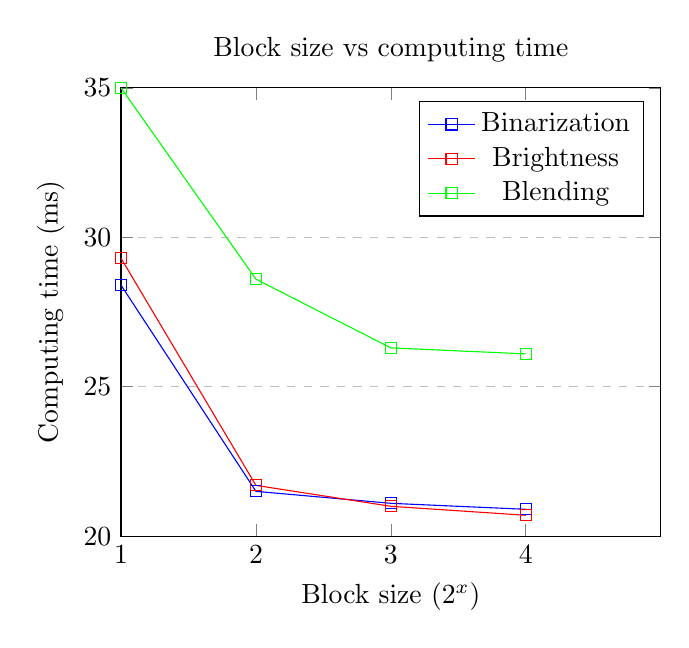
\begin{tikzpicture}
        \centering
        %%define axes
        \begin{axis}[
            title={Block size vs computing time},
            xlabel={Block size ($2^x$)},
            ylabel={Computing time (ms)},
            xmin=1, xmax=5,
            ymin=20, ymax=35,
            xtick={1, 2, 3, 4},
            ytick={20, 25, 30, 35},
            legend pos=north east,
            ymajorgrids=true,
            grid style=dashed,
        ]
        %% data filing
        \addplot[color=blue, mark=square]
            coordinates { %% Remind : axis X = 2^x
                (1,28.4)(2,21.5)(3,21.1)(4,20.9)
            };
        \addplot[color=red, mark=square]
            coordinates { %% Remind : axis X = 2^x
                (1,29.3)(2,21.7)(3,21.0)(4,20.7)
            };
        \addplot[color=green,mark=square]
            coordinates { %% Remind : axis X = 2^x
                (1,35)(2,28.6)(3,26.3)(4,26.1)
            };
        
        \legend{Binarization, Brightness, Blending}
        \end{axis}
    \end{tikzpicture}
    \newline


\end{document}

